\section{Production traffic}
\label{sec:production}

Synthetic sessions let us place the cliff; they do not say whether production traffic ever reaches it. The Kimi
tool-agent trace (Section~\ref{sec:setup}) answers that for one large deployment. Two of its properties matter. With
an unbounded cache, 55\% of its prompt blocks are reused, close to the 54--62\% Wang et~al.\ report for Alibaba's
traces~\cite{wang2025kvcachewild}. And requests in the same conversation return after a median of 114\,s (90th
percentile 420\,s): the gaps between a conversation's requests, which include tool
time, generation and queueing, last minutes, not the 5--30\,s pauses of our synthetic runs.

\paragraph{The host tier serves what the GPU cannot.} At a 1/4 sample (1,363 requests in the first window, 1,542 in the
second, about 11.5--12.2k prompt tokens per second) one H200 is past its capacity even with a cache
(Table~\ref{tab:prod}, Figure~\ref{fig:production}). With the GPU cache alone it finished 85--86\% of requests within the window plus 240\,s, with a
median TTFT of 89--200\,s; without a cache, 61--62\%. With a 160\,GB SGLang host tier it finished
every request in both windows, at 15--17\% less energy per prompt token than the GPU cache alone and about 40\% less than
no cache. The card averaged 585--590\,W under every policy, so total GPU energy over the window differed by at most
3.3\% between no cache, the GPU cache and the 160\,GB tier: the tier's gain is 16--18\% more prompt tokens finished for about the same energy, a gain in capacity. At the
1/8 sample, where every policy finished every request, the 160\,GB tier used 85.54\,mJ per prompt token against 86.08
for vLLM's GPU cache ($-0.6\%$; no SGLang GPU-cache run at 1/8). In the first window at 1/4, vLLM and SGLang with the GPU cache alone agreed to 0.1 points in hit rate and 1\% in energy, and the 160\,GB result
repeated within 0.1\% in a second round. A 300\,GB tier raised the hit rate by three more points, lowered energy by
another 4\% and cut the median TTFT from 129\,s to 107\,s.

\begin{table}[t]
\centering\small
\caption{Replay of Kimi's production tool-agent trace on one H200 (Qwen3-32B), 1/4 of the trace, 15-minute windows.
Done: requests finished within the window plus 240\,s. mJ/tok: all GPU energy of the window and drain divided by the prompt tokens of finished requests, which counts partial
work on unfinished requests and so raises the values of the policies that left requests unfinished. TTFT: median time to first token. Tiers are SGLang host tiers. Window: minutes of the trace replayed. Hit: prompt-token hit rate. Values are from one round; three first-window cells were repeated, and the repeats agreed within 0.2\% in energy and hit rate and 0.3\% in TTFT.}
\label{tab:prod}
\begin{tabular}{llrrrr}
\toprule
Window & Policy & Done & Hit & mJ/tok & TTFT \\
\midrule
0--15 & no cache (vLLM) & 61\% & 0\% & 104.4 & 270\,s \\
0--15 & GPU (vLLM) & 86\% & 36.7\% & 74.8 & 200\,s \\
0--15 & GPU (SGLang) & 86\% & 36.6\% & 75.6 & 199\,s \\
0--15 & 160\,GB (SGLang) & 100\% & 51.8\% & 62.8 & 129\,s \\
0--15 & 300\,GB (SGLang) & 100\% & 54.8\% & 60.3 & 107\,s \\
30--45 & no cache (vLLM) & 62\% & 0\% & 101.6 & 236\,s \\
30--45 & GPU (vLLM) & 85\% & 38.2\% & 71.9 & 89\,s \\
30--45 & 160\,GB (SGLang) & 100\% & 52.2\% & 61.3 & 67\,s \\
\bottomrule
\end{tabular}
\end{table}

\begin{figure}[t]
\centering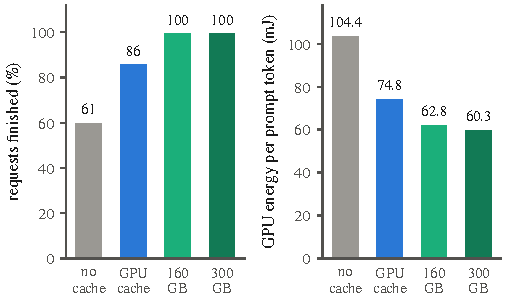
\includegraphics[width=\columnwidth]{../figures/production.pdf}
\caption{Kimi tool-agent trace, 1/4 sample, first window, one H200. Left: share of requests finished; right: GPU energy per
prompt token, which includes energy spent on unfinished requests (round 1, the values of Table~\ref{tab:prod}). No cache and GPU cache on vLLM; host tiers on SGLang.}
\label{fig:production}
\end{figure}

\paragraph{The energy model on production traffic.} Equation~\eqref{eq:energy}, with the $f=0.76$ fitted on synthetic
sessions, predicts the ratio of each policy's energy per prompt token to that of no cache from its measured hit rate.
On the busy card it is right to within about 1\%: 0.721 predicted against 0.717--0.718 measured for vLLM's GPU cache, 0.606
against 0.601 for 160\,GB and 0.584 against 0.578 for 300\,GB in the first window, and 0.709 against 0.708 for the GPU cache and 0.603 against 0.603 for 160\,GB
in the second. At a 1/8 sample, where the GPU cache ran well below full power (544\,W), the model fails: the GPU cache measured 0.847 of no-cache
energy where the model gives 0.653. There the window includes idle and decode-bound time, the prefill share is smaller
(the measured ratio implies $f\approx0.33$), and the cache's benefit is mostly latency: a median time to first token of
1.2\,s instead of 18\,s, and a 90th percentile of 7.1\,s instead of 77\,s.

\paragraph{Predicting the hit rate from logs.} Because the trace carries block hashes, the hit rate of any cache size
can be estimated offline by replaying the hashes through an LRU of that many blocks, as KVSET does with the Mattson
stack algorithm~\cite{kvset2026,mattson1970evaluation}. We wrote these predictions before each run. When the card kept
up (finished every request), they came within 0.6 points at 1/8 and 2.3--4.3 points at 1/4: 45.65\% measured against 46.25\% predicted for the GPU cache at 1/8 in the second window, 52.62\%
against 52.66\% for 160\,GB at 1/8, and 51.8\% and 54.8\% against 47.5\% and 52.5\% for 160 and 300\,GB at 1/4 in the first. When
the card was overloaded the predictor read high: 36.7\% measured against 41.8\% predicted, and 38.2\% against 44.7\%,
for the GPU cache alone at 1/4. A likely cause, which we did not measure, is that unfinished requests and queueing change which requests the cache
sees and in what order; a prediction from logs must therefore come with a capacity check.

From hashed request logs alone, which contain no prompt text, one can estimate what hit rate a given GPU and host
memory will reach when the card keeps up and, on a busy card, what that hit rate will save in energy. Chained, the
logged hit-rate prediction and Eq.~\eqref{eq:energy} put the two host tiers at 1/4 in the first window within 4--6\% of their measured
energy ratios.
